\chapter{Method}
\section{Radial velocity components in linear theory}\label{sec:radlintheory}
One of the goals of this project is to test the viability of using the assumptions
from linear theory and study wether it is a good physical approximation for
studying the physics of voids and filaments. The radial velocity component of
halos in filaments and voids is an analytical tool that is useful for comparing
with data from simulation for testing wether linear theory can be used to
approximate the physical behaviour of halos and galaxies observed in these objects.
\subsection{Radial velocity component for filaments}
When calculating the radial velocity component of filaments, the average filament is
approximated to be a cylindrical object. The radial component is the component of
the velocity vector $\vec{v}$ that points perpendicular to the longitudinal axis
$L$. This is illustrated in figure \ref{fig:filamentvr}. For this analysis we
will assume that the other velocity components are negligible and that the
radial component is the significant component.
\begin{figure}\label{fig:filamentvr}
    \begin{tikzpicture}
        \draw[->] (-4,0,0) -- (4,0,0) node[below right] {$L$};
        \draw[->] (0,1,0) -- (0,0.5,0) node[below right] {$v_r$};
        \draw[->] (0,-1,0) -- (0,-0.5,0) node[below right] {$v_r$};
        \node (A) [draw, cylinder, shape aspect=1.8, minimum height=50mm, minimum width=20mm] {};
    \end{tikzpicture}
    \caption{Illustration of a cylindrical filament with longitudinal axis $L$ and radial velocity component $v_r$.}
\end{figure}
in linear theory can be written as
\begin{equation}\label{eq:lincont}
    \frac{d\delta}{dt}+\frac{1}{a}\nabla\cdot\vec{v}=0.
\end{equation}
 The continuity equation In linear theory one can write
 $d\delta/dt=Hf\delta$ \cite[p.~347]{schneider2006extragalactic}, where $f$ is the growth factor
defined in equation \ref{eq:growthfac}. Substituing this into equation
\ref{eq:lincont} one will get
\begin{equation}\label{eq:templineq}
    \nabla\cdot\vec{v}=-Hfa\delta.
\end{equation}
Assuming cylindrical coordinates we can replace the
divergence
\begin{equation}
    \nabla\cdot\vec{v}=\frac{1}{r}\frac{\partial}{\partial r}(rv_r)+\frac{1}{r}\frac{\partial v_\phi}{\partial \phi} +\frac{\partial v_L}{\partial L}.
\end{equation}
Assuming that the radial component $v_r$ gives the significant contribution and
the two other are negligible, by inserting into equation \ref{eq:templineq} on
will get
\begin{equation}
    \frac{1}{r}\frac{\partial}{\partial r}(rv_r)=-Hfa\delta.
\end{equation}
Multiplying both sides by $r$ and integrating one will be left with
\begin{equation}
    v_r=-\frac{1}{r}Hfa\int_0^r\delta(x) x dx.
\end{equation}
By defining the average mass density contrast for filaments $\Delta_f(r)$
as
\begin{equation}\label{eq:contrastfil}
    \Delta_f(r)=\frac{2}{r^2}\int_0^r\delta(x) x dx,
\end{equation}
one can write the radial velocity component for a halo in a filament as
\begin{equation}\label{vrfilament}
    v_r(r) = -\frac{1}{2}Hfar\Delta_f(r).
\end{equation}
\subsection{Radial velocity component for voids}
The radial velocity component for voids is similar to the one for filaments
except that for voids one assumes a spherical coordinate system. This assumption
is based on the notion that the average void should have a spherical shape with,
on average, no prefferred direction for overdensities on the rim and
thereby having a spherical density profile. Since objects cluster towards larger
densities, approximating the velocity of halos and galaxies around
voids to be dominated by the radial component, moving straight away from the
underdensity in the center of the void one can argue that the radial velocity
should be the dominating component. This is illustrated in figure \ref{fig:filamentvr}.
\begin{figure}\label{fig:filamentvr}
    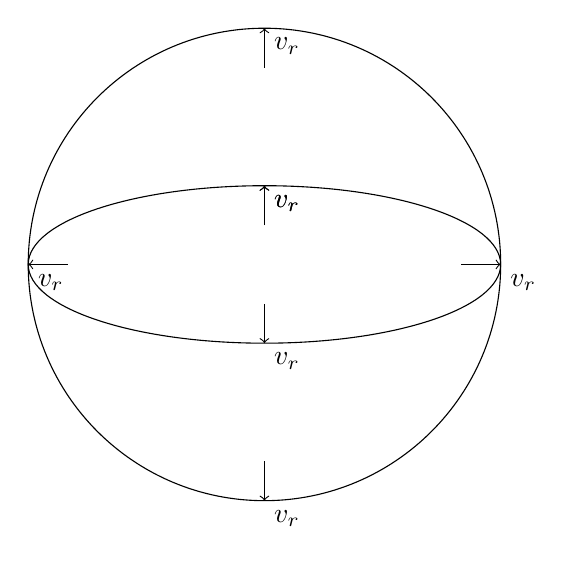
\begin{tikzpicture}
        \draw[->] (0,0.5,0) -- (0,1,0) node[below right] {$v_r$};
        \draw[->] (0,-0.5,0) -- (0,-1,0) node[below right] {$v_r$};
        \draw[->] (0,0.5,0) -- (0,1,0) node[below right] {$v_r$};
        \draw[->] (2.5,0,0) -- (3,0,0) node[below right] {$v_r$};
        \draw[->] (-2.5,0,0) -- (-3,0,0) node[below right] {$v_r$};
        \draw[->] (0,2.5,0) -- (0,3,0) node[below right] {$v_r$};
        \draw[->] (0,-2.5,0) -- (0,-3,0) node[below right] {$v_r$};
        \draw (0,0) circle (3cm);
        \draw (0,0) ellipse (3cm and 1cm);
    \end{tikzpicture}
    \caption{Illustration of a spherical void with radial velocity pointing outwards from the center of the void.}
\end{figure}
The derivation for the radial velocity component is the same for voids as for
filaments up until equation \ref{eq:templineq}. The difference for voids is that
the divergence now has to be calculated in spherical coordinates given by
\begin{equation}
    \nabla\cdot \vec{v}=\frac{1}{r^2}\frac{\partial}{\partial r}(r^2v_r)
                       +\frac{1}{r\mathrm{sin}\theta}\frac{\partial}{\partial r}(\mathrm{sin}\theta v_\theta)
                       +\frac{1}{r\mathrm{sin}\theta}\frac{\partial}{\partial r}(\phi v_\phi).
\end{equation}
As for filaments only the radial component is assumed to be non-negligible
giving
\begin{equation}
    \frac{1}{r^2}\frac{\partial(r^2v_r)}{\partial r}=-Hfa\delta.
\end{equation}
Multiplying by $r^2$ and integrating one will get
\begin{equation}
    v_r = -\frac{1}{r^2}Hfa\int_0^r x^2\delta(x)dx.
\end{equation}
As for filaments a average mass density contrast for voids is defined as
\begin{equation}\label{eq:contrastvoid}
    \Delta_v(r)=\frac{3}{r^3}\int_0^r x^2\delta(x)dx,
\end{equation}
which will give an expression for the radial velocity for voids
\begin{equation}\label{eq:vrvoid}
    v_r(r)=-\frac{1}{3}Hfar\Delta_v(r).
\end{equation}
\section{Numerical measurement of correlation functions and multipole expansions.}
As mentioned in section \ref{sec:corrtheory} correlation functions are useful
tools for measuring the statistical properties of the universe. In order to test
analytical models one has to compare with data from observations or simulations.
The code \footnote{The code for measuring correlation functions utilized for this analysis can be found at \url{https://github.com/seshnadathur/pyCUTE}.} used for this project to measure angular correlation functions
implements a Landy-Szalasay estimator \cite{Landy}. The Landy-Szalasay estimator
for the angular cross correlation function, where $s$ denotes redshiftspace, reads
\begin{equation}
    \xi^s(s,u)=\frac{\langle D_1D_2\rangle-\langle D_1R_2\rangle-\langle D_2R_1\rangle+\langle R_1R_2\rangle}{\langle R_1R_2\rangle}.
\end{equation}
Where, in this analysis, subscript $1$ denotes either void centers or center or
the center of cosmic filaments and subscript $2$ denotes halo positions. $D_1$
and $D_2$ refers to the actual data while $R$ is samples from a random
distribution resembling the dataset. Each quantity in the squared brackets
denote the mean value of of a pair with separation $r$ and $\mu$, where
$\mu=cos(\theta)$ is the cosine of the angle between the separation vector and
the line of sight direction. An illustration of a pair in the coordinate system
of the observer is illustrated in figure \ref{fig:corrpair}
\begin{figure}\label{fig:corrpair}
    \begin{tikzpicture}
        \def\myrad{2}% radius of the circle
        \def\myang{60}% angle for the arc
        %\draw (0,0) -> (10,0) {s};
        % the origin
        \coordinate (O) at (10,0);
        
        \draw[line width=0.2mm][->] (0,0) -- (10,0);
        \draw[line width=0.2mm][->] (10,0) -- (10-1.414,-1.414);
        % the circle and the dot at the origin
        \node[text width=10cm] at (13.3,0.5) {Filament/void center};
        \node[text width=10] at (5,0.5) {$\vec{s}$};
        \node[text width=10] at (9,-1.4) {$\vec{r}$};
        \node[text width=5] at (0,1) {Observer};
        \node[text width=5] at (10-1.3*0.93,-1.3*0.34) {$\theta$};
        \draw (O) node[circle] {} circle [radius=\myrad];
        % the ``\theta'' arc
        \draw (O) [thick,domain=180:225] plot ({10 + cos(\x)}, {sin(\x)});
    \end{tikzpicture}
    \caption{Figure illustrating the system where pairs are counted for the angular cross correlation function. Sjekk opp om S egentlig skal være r}
\end{figure}
\\\indent
In order to remove the angular dependency, the angular correlation function is
expanded in mulitpoles. The multipoles are given by 
\begin{equation}
    \xi^s_\ell(s)=\int_0^1\xi^s(s,\mu)(1+2\ell)L_\ell(\mu)d\mu
\end{equation}
\cite{Nadathur_corr}, where $L_\ell(\mu)$ are Legendre polynomials
of order $\ell$. In this analysis only the monopole and multipole
are taken into consideration. The Legendre multipoles for $\ell=0$ and
$\ell=1$ are given by
\begin{equation}
    L_0(\mu)=1
\end{equation}
and
\begin{equation}
    L_2(\mu)=(3\mu^2-1)/2.
\end{equation}
\section{Void Analysis}
\subsection{Density profile}\label{sec:voiddensity}
After running the void finding algorithm from REVOLVER on our dataset we have a list of $x$, $y$
and $z$ coordinates for every void center. With a catalogue of void centers one
has to compare their position to the galaxy catalogue in which they are found to
calculate the average density profile as a function of distance from the void
center. Using a periodic kd-tree module \footnote{The periodic kd-tree code
applied for this analysis is found at at \url{https://github.com/patvarilly/periodic_kdtree}} to search for
the nearest halos of the void centers with a gradually increasing radius one can count the halos in
the catalogue close to a given void center. For every void a search for
neghbouring halo particles is conducted with a gradually increasing radius. For
a linearly spaced radius array $\vec{r}=\{r0,\dots,r_{n}\}$ using an iterative
approach every galaxy in a sphere with radius $r_{i}$, where
$i\in\mathbb{N}\bigcap [r_0,r_{n}]$ denotes the
number of iterations, is counted. The total number of halos is stored for
every iteration. For the first iteration the number of halos in a sphere around the void
center is calculated and stored. The density for this sphere is then $n_i/V_i$,
where $n_i$ is the number of halos inside the sphere and $V_i=4\pi r_{i}^3/3$. For
the next iteration the number of halos inside a sphere with radius $r_{i+1}$ is
counted. Alot of the halos inside this new sphere overlaps with the previous
sphere. Therefore the number of halos in the previous step were stored and then
subtracted from the number of galaxies in the new sphere leaving only the number
of halos counted in the spherical shell that does not overlap between the two
spheres. The volume of this spherical shell is $V_{i+1}=4\pi(r_{i+1}^3-r_i^3)/3$. The
number density in the shell defined by subtracting the previous sphere from the
new sphere is the number of galaxies in the new sphere subtracted by the number
of galaxies in the previous sphere divided by the volume of the sperical shell.
The total number of galaxies in the new sphere is stored and this process is
repeat for all iterations defined by the radius vector $\vec{r}$. This process
will give the density profile as a function of radius for a given void. By
adding the density profiles for all voids and diving by the number of voids one
will get an average density profile for the whole dataset.
\subsection{Velocity profile and velocity dispersion}
When studying linear theory applied to voids and filaments, one needs an observational or
numerical representation to test its validity. As explained in section
\ref{sec:radlintheory} the radial velocity profile can be represented analytically and
may provide a good comparison. In addition to the $x$, $y$ and $z$ coordinates for the
halo particles, the galaxy catalogue used also containts the $v_x$, $v_y$ and
$v_z$ particles. The radial velocity profile is calculated in a
similar manner as the density profile for voids described in
\ref{sec:voiddensity}. Using a periodic kd-tree centered at the current void one
can count all particles in a sphere around the current void center. For a given
halo particle its position with respect to a given void center is given by
\begin{equation}\label{eq:voidpos}
    \vec{r}=\vec{r}_{\mathrm{void}}-\vec{r}_{\mathrm{halo}}.
\end{equation}
This is the vector that points radially from the void center to a given halo
particle. The radial velocity component is is the component of the velocity of a
given halo particle $\vec{v}$ that points along this vector. The component of vector
$\vec{v}$ along vector $\vec{r}$ is caluclated as
\begin{equation}
    v_r=\frac{\vec{r}\cdot\vec{v}}{\vert\vec{r}\vert}.
\end{equation}
This is the radial velocity for a halo particle with respect to a given void
center. In a similar manner to the density profile the radial velocity is
calculated iteratively for every particle in sphere around the void center. In
order to get the radial velocity profile the particles are divided into
shells. For every iteration, for a given void, for each sphere the radial
velocity is stored for the next iteration. The radial velocity in a given shell
for the next iteration is the radial velocity in the new sphere subtracted by
the radial velocity in the previous sphere. This is averaged by, for each shell,
dividing by the number of particles in a given shell. After this has
been done for all voids the radial velocity profile is divided by the number of voids in the catalogue to get
the average radial velocity profile for a single halo particle in the catalogue.
\\\indent
The velocity dispersion $\sigma_v$ is also calculated. The velocity dispersion
is given by the usual expression for the standard derivation
\begin{equation}
    \sigma_{v} = \sqrt{\langle v^2 \rangle + \langle v\rangle^2}.
\end{equation}
This velocity is along the line of sight for the observer. For the multidark
dataset this is along the $z$ direction and therefore only the $v_z$ component
is considered. This is calculated in spherical shells around each void center to
get the average void velocity dispersion profile.
\subsection{Void-galaxy cross correlation function.}
As mentioned in section \sec{sec:corrtheory} cross correlation functions are
essential tools in cosmology for measuring the statistical properties of
observables in the universe. In this analysis one of the cross correlations that
will be looked into is the cross correlation between void centers and galaxies
or halos. Following the approach of \cite{Nadathur_corr}, the following
subsection will describe how to derive the void-galaxy cross correlation
function. 
\\\indent
Let $\vec{r}_{void}$ denote the position of a void center and $\vec{r}_{halo}$ denote the
position of a halo or galaxy particle in realspace. Their separation vector $\vec{r}$ is then
given by equation \ref{eq:voidpos}. The relation from redshiftspace to realspace
can be written as
\begin{equation}
    \vec{s}=\vec{r}+\frac{\vec{v}_{pec}\cdot\hat{r}_{void}}{aH}\hat{r}_{void},
\end{equation}
where $v_{pec}$ is the peculiar velocity of a galaxy or halo particle and
$\hat{r}_{void}=\vec{r}_{void}/ \vert \vec{r}_{void}\vert$. Here it is assumed
that the velocity of void centers are negligible. The number of voids in
realspace may not be preserved in redshiftspace. Therefore reconstruction,
described here in section \ref{sec:reconstrction}, has to be applied to regain
the field in realspace from redshiftspace. The basic assumption
required is that the number of void-galaxy pairs in the simulation volume is
unchanged during transformation from realspace to redshiftspace. This is stated
mathematically as
\begin{equation}
    (1 + \xi^s_{\mathrm{vg}}(\vec{s}))\mathrm{d}^3\mathrm{s}=(1 + \xi^r_{\mathrm{vg}}(\vec{r}))\mathrm{d}^3\mathrm{r},
\end{equation}
where superscript $r$ and $s$ denotes realspace and redshiftspace respectively.
Here $\xi^s_{vg}(\vec{s})$ is the cross correlation between realspace voids and
the redshifted galaxy field and $\xi^r_{vg}(\vec{r})$ is the cross correlation
between realspace voids and realspace galaxy positions. Another assumption made
is that the velocity of all halo particles near a void can be approximated by
its radial velocity $\vec{v}=v_r \hat{r}$, where $\hat{r}$ is the radial unit vector
in a spherical coordinate system. The Jacobian of the